A continuación veremos las \textbf{dApps} más conocidas a día de hoy en los
distintos ámbitos principales[\cite{aplicaciones-descentralizadas}]: Redes
sociales, Servicios de intercambio monetario, servicios de almacenamiento,
Servicios de \textit{streaming} de vídeo y música

\label{dApps}
\subsection*{Redes Sociales Web3}
\label{webs-socialNetworks}
\textbf{Steemit}[\url{https://steemit.com}]: Se ejecuta completamente en la blockchain
Steem. Se describe mejor como una plataforma de recompensa descentralizada que
ayuda a los contribuyentes a monetizar su contenido. Es una alternativa a
Reddit[\url{https://reddit.com}].
\begin{figure}[htb!]
    \caption{Logo de Steemit}
    \label{fig:steemit}
    \centering
    
\includegraphics[scale=0.30]{./Ilustraciones/logos/steemit-logo.png}\\
    \textbf{Fuente:} Steemit[\url{https://steemit.com}]
\end{figure}
Beneficios de las redes sociales descentralizadas. Ninguna autoridad central
que capture datos y los use. Empodera a los usuarios al recompensarlos con
algún tipo de activo. Mejora en las redes sociales de la Web 2.0 en casi todos
los sentidos. Protege la privacidad de los usuarios. Los usuarios deciden qué
quieren compartir y cuándo. Las grandes corporaciones y organizaciones pierden
poder para influir en las grandes corporaciones.

\subsection*{Servicios de intercambio descentralizados}
\label{webs-finanzas}
Cualquiera de estas aplicaciones podrían asociarse a lo que podría ser un
banco, donde podemos introducir dinero en distintas divisas, realizar
transacciones, y el precio de las distintas divisas.

\hfill \break
\textbf{IDEX}: Es un servicio de intercambio descentralizado popular para el
comercio de tokens ERC-20. Proporciona una buena interfaz para los usuarios,
y, cualquier persona con una cartera de ethereum puede comenzar a operar en
la plataforma. Para hacer el mejor uso de IDEX o de cualquier intercambio
descentralizado basado en ethereum, debes utilizar MetaMask.

\hfill \break
\textbf{Coinbase}: Es una plataforma de intercambio de criptomonedas en línea
que permite a los usuarios comprar, vender y almacenar una variedad de
criptomonedas, como Bitcoin, Ethereum, Litecoin, entre otras. Fue fundada en
2012 y se ha convertido en una de las plataformas más populares y utilizadas
en el mundo de las criptomonedas.
\begin{figure}[htb!]
    \caption{Logo de Coinbase}
    \label{fig:coinbase-logo}
    \centering
    
\includegraphics[scale=1]{./Ilustraciones/coinbase-logo.png}\\
    \textbf{Fuente:} Coinbase[\url{https://www.coinbase.com}]
\end{figure}
Además de la plataforma de intercambio, Coinbase también ofrece una billetera
digital integrada para almacenar las criptomonedas y una API para
desarrolladores que deseen integrar las funcionalidades de la plataforma en sus
propias aplicaciones.

\hfill \break
Una de las principales características de Coinbase es su interfaz de usuario
intuitiva y amigable, lo que la hace atractiva tanto para principiantes como
para usuarios avanzados. También se ha destacado por su enfoque en la seguridad
y la protección de los activos de los usuarios, utilizando medidas de seguridad
avanzadas como la autenticación de dos factores y la custodia de criptomonedas.

\hfill \break
Hacer intercambios de criptomonedas de forma descentralizada tiene ciertos
beneficios:
\begin{itemize}
    \item Transacciones más baratas.
    \item Transacciones más rápidas.
    \item Difícil de piratear debido a la naturaleza descentralizada.
    \item Funciona bien con carteras de hardware.
    \item Los usuarios controlan sus propios fondos.
\end{itemize}
Sin embargo, los intercambios descentralizados no están libres de negativos.
Pueden ser difíciles de usar y comprender para los usuarios. Además, la
generación actual de intercambios descentralizados también sufre la falta de
características y funcionalidades. Sin embargo, con el tiempo, veremos la red
descentralizada más avanzada a la par con las contrapartes centralizadas.

\hfill \break
\subsection*{Servicios de Almacenamiento descentralizados}
\label{webs-almacenamiento}
Las siguientes herramientas podrían ser comparadas en la Web2 con Dropbox, Google
Drive o Microsoft OneDrive.

\hfill \break
\textbf{Storj}[\url{https://www.storj.io}]: Storj es una de las principales soluciones de almacenamiento
descentralizado. También es uno de los más antiguos. Con Storj, cualquiera
puede almacenar datos. También es de código abierto y fácil de usar. Cualquiera
puede comenzar a utilizarlo con solo 1-Clic en Inicio. El modelo de pago se
crea alrededor de los usuarios, ya que pueden pagar según lo utilicen. El token
Storj se utiliza para alimentar la plataforma Storj.

\hfill \break
\textbf{Sia}[\url{https://sia.tech}]: Proporciona almacenamiento de forma descentralizada
y también se considera la mayor competencia de Storj. Sia divide el
archivo en treinta segmentos y luego lo distribuye. También encripta el archivo
mientras se transfiere.
\begin{figure}[htb!]
    \caption{Logo de Sia}
    \label{fig:sia}
    \centering
    
\includegraphics[scale=0.25]{./Ilustraciones/logos/sia-logo.jpg}\\
    \textbf{Fuente:} Steemit
\end{figure}
\textbf{IPFS (InterPlanetary File System)}[\url{https://ipfs.tech}]: Es una tecnología de
almacenamiento distribuido que utiliza la red blockchain para almacenar
archivos de manera descentralizada. IPFS permite a los usuarios acceder a los
archivos de forma más rápida y segura, ya que los archivos se almacenan en
múltiples nodos en la red.
\begin{figure}[htb!]
    \caption{Logo de IPFS}
    \label{fig:ipfs}
    \centering
    
\includegraphics[scale=0.25]{./Ilustraciones/logos/ipfs-logo.jpg}\\
    \textbf{Fuente:} wikipedia [\url{https://es.wikipedia.org/wiki/Sistema_de_archivos_interplanetario}]
\end{figure}
Beneficios de las soluciones de almacenamiento descentralizado Funciona bien en
diferentes plataformas o incluso en soluciones de blockchain. Protege los datos
que se transfieren con cifrado fuerte. Ninguna entidad centralizada, significa
que nadie puede usar los datos. Es barato y funciona bien con tecnologías de
próxima generación como \textbf{IoT (Internet de las cosas)}.

\hfill \break
\subsection*{\textit{Streaming} de Vídeo y Música} \label{webs-streaming} Aquí podríamos comparar con
apliaciones como Twitch[\url{https://www.twitch.tv}],
YouTube[\url{https://www.youtube.com}] o U-beat[\url{https://ubeat.tv}], en el
apartado de \textit{streaming} de vídeo, y aplicaciones web como YouTube
Music[\url{https://music.youtube.com}],
Spotify[\url{https://open.spotify.com/}], o
SoundCloud[\url{https://soundcloud.com}], para el \textit{streaming} de música.

\hfill \break
\textbf{LivePeer}[\url{https://livepeer.org/es}]: Proporciona un servicio de
transmisión, es de código abierto y apunta a construir una stack de streaming
para la Web 3.0.

\hfill \break
\textbf{LBRY}[\url{https://lbry.com}]: Biblioteca digital
descentralizada que alberga diferentes formas de contenido. Como usuario,
puedes leer, ver y jugar en la plataforma. Esto significa que admite libros,
música y videos. Es uno de los proyectos Web 3.0 más antiguos.

\hfill \break
\textbf{UjoMusic}[\url{https://www.mesh.xyz}]: Plataforma de música donde los
creadores pueden cargar su música y distribuirla sin problemas de derechos de
autor o royalty. Las criptomoneda y los contratos inteligentes lo potencian.

\hfill \break
\textbf{Audius}[\url{https://audius.co}]: Es una plataforma de música
descentralizada que permite a los artistas compartir su música y monetizarla.
Los usuarios pueden escuchar música de forma gratuita. Esta aplicación es la
que pretende reemplazar a Spotify dentro del mundo descentralizado.

\begin{figure}[htb!]
    \caption{Logo de Audius}
    \label{fig:audius}
    \centering
    
\includegraphics[scale=0.25]{./Ilustraciones/logos/Audius.jpg}\\
    \textbf{Fuente:} Ecosystem.ipfs [\url{https://ecosystem.ipfs.tech/project/audius/}]
\end{figure}

\hfill \break
Los creadores de contenido pueden trabajar en un entorno transparente. odos
tienen las mismas oportunidades de promover su trabajo. Los problemas de
derechos de autor serán insignificantes gracias a los contratos inteligentes y
no hay autoridad central, por lo tanto no será una política absurda para los
streamers y los creadores de contenido.

\subsection*{Navegadores descentralizados}
\label{webs-browsers}
Teniendo en cuenta los navegadores más utilizados en estos últimos 5 años [Figura \ref{fig:browser}],
podemos ver que las comparaciones son abrumadoras, teniendo Google Chrome casi un 63\% del mercado,
siguiéndole Safari, Mozilla Firefox y Samsung Internet.
Por lo que cualquiera de los siguientes navegadores no pueden competir con este,
aunque tienen sus beneficios al estar implementando la tecnología blockchain.

\hfill \break
\textbf{Brave Browser}[\url{https://brave.com/es/}]:
Brave tiene que ver con la privacidad donde los usuarios no son el producto.
El navegador viene preinstalado con el bloqueador de anuncios. También permitirá
a los usuarios vender sus datos a cambio de la criptomoneda, BAT, la cual pueder
ser usada para diversos propósitos, como pueden ser hacer Staking, ser cambiadas por
otra Criptomoneda, o venderla para conseguir divisa.

\begin{figure}[htb!]
    \caption{logos de Brave}
    \label{fig:brave}
    \centering
    
\includegraphics[scale=0.1]{./Ilustraciones/logos/brave-logo.png}\\
    \textbf{Fuente:} logos.Wine
\end{figure}

\textbf{Breaker Browser}[\url{https://github.com/beakerbrowser}]:
Es un navegador web de próxima generación basado en
punto a punto (P2P)\footnote{ red de computadoras en la que todos los aspectos
    (o la mayoría de ellos) funcionan con una serie de nodos que se comportan de
    la misma manera entre sí y sin clientes ni servidores fijos\cite{p2p}}.
Es un lugar donde cualquiera puede unirse, compartir y
sobrecargar sus aplicaciones. Es una herramienta creativa que puede ser
explorada por cualquier persona. Es un navegador web 3.0.

\hfill \break
Beneficios de los navegadores descentralizados: Los usuarios pueden navegar de
forma privada por internet.\\ Ninguna o menor cantidad de lagunas de seguridad.
\\ Los usuarios pueden vender sus datos a una organización y recibir pagos.
Rápido y seguro.
\begin{figure}[htb!]
    \caption{Navegadores más usados entre 2018 y 2023}
    \label{fig:browser}
    \centering
    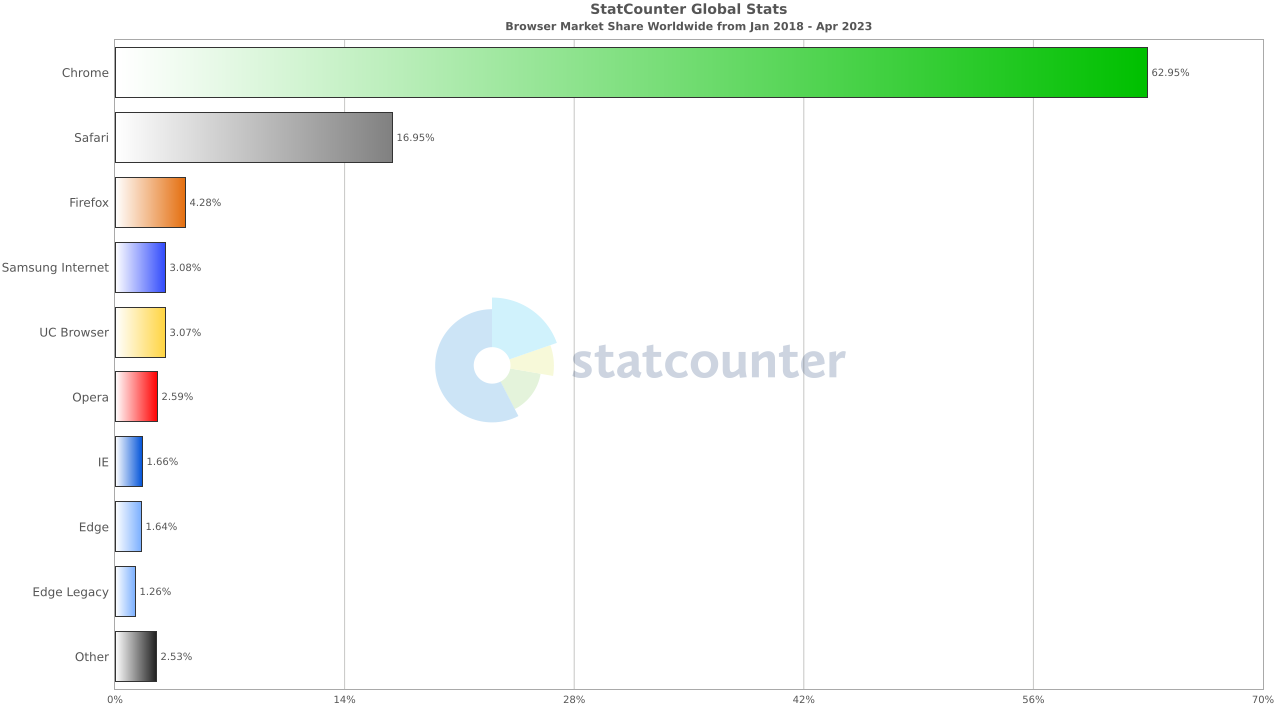
\includegraphics[scale=0.5]{./Ilustraciones/StatCounter-browser-ww-monthly-201801-202304-bar.png}\\
    \textbf{Fuente:} StatCounter [\url{https://gs.statcounter.com/browser-market-share#monthly-201801-202304-bar}]
\end{figure}